The goal of the design of cloud deployments was to be cloud agnostic, meaning it should work with any cloud provider with minimal/no changes. For that reason, all services are meant to be deployed in a Kubernetes cluster, but the location or structure of the cluster doesn't matter. All of the biggest cloud providers have Kubernetes as a Service (KaaS) offering moreover it is very common along smaller providers as well.

The overall design of the cloud services can be seen in figure \ref{fig:cloud_services}. Services are communicating with each other in two ways:
\begin{itemize}
    \item Via Cloud broker - Backend and Cloud-Agent are both subscribed to a series of topics and exchange information through MQTT messages sent to the cloud broker. 
    \item Via REST endpoints - Backend services expose the REST endpoint which is consumed by Frontend. Frontend itself is only meant to serve HTML documents and be a consumer of the backend endpoint.
\end{itemize}

\begin{figure}[H]
    \centering
    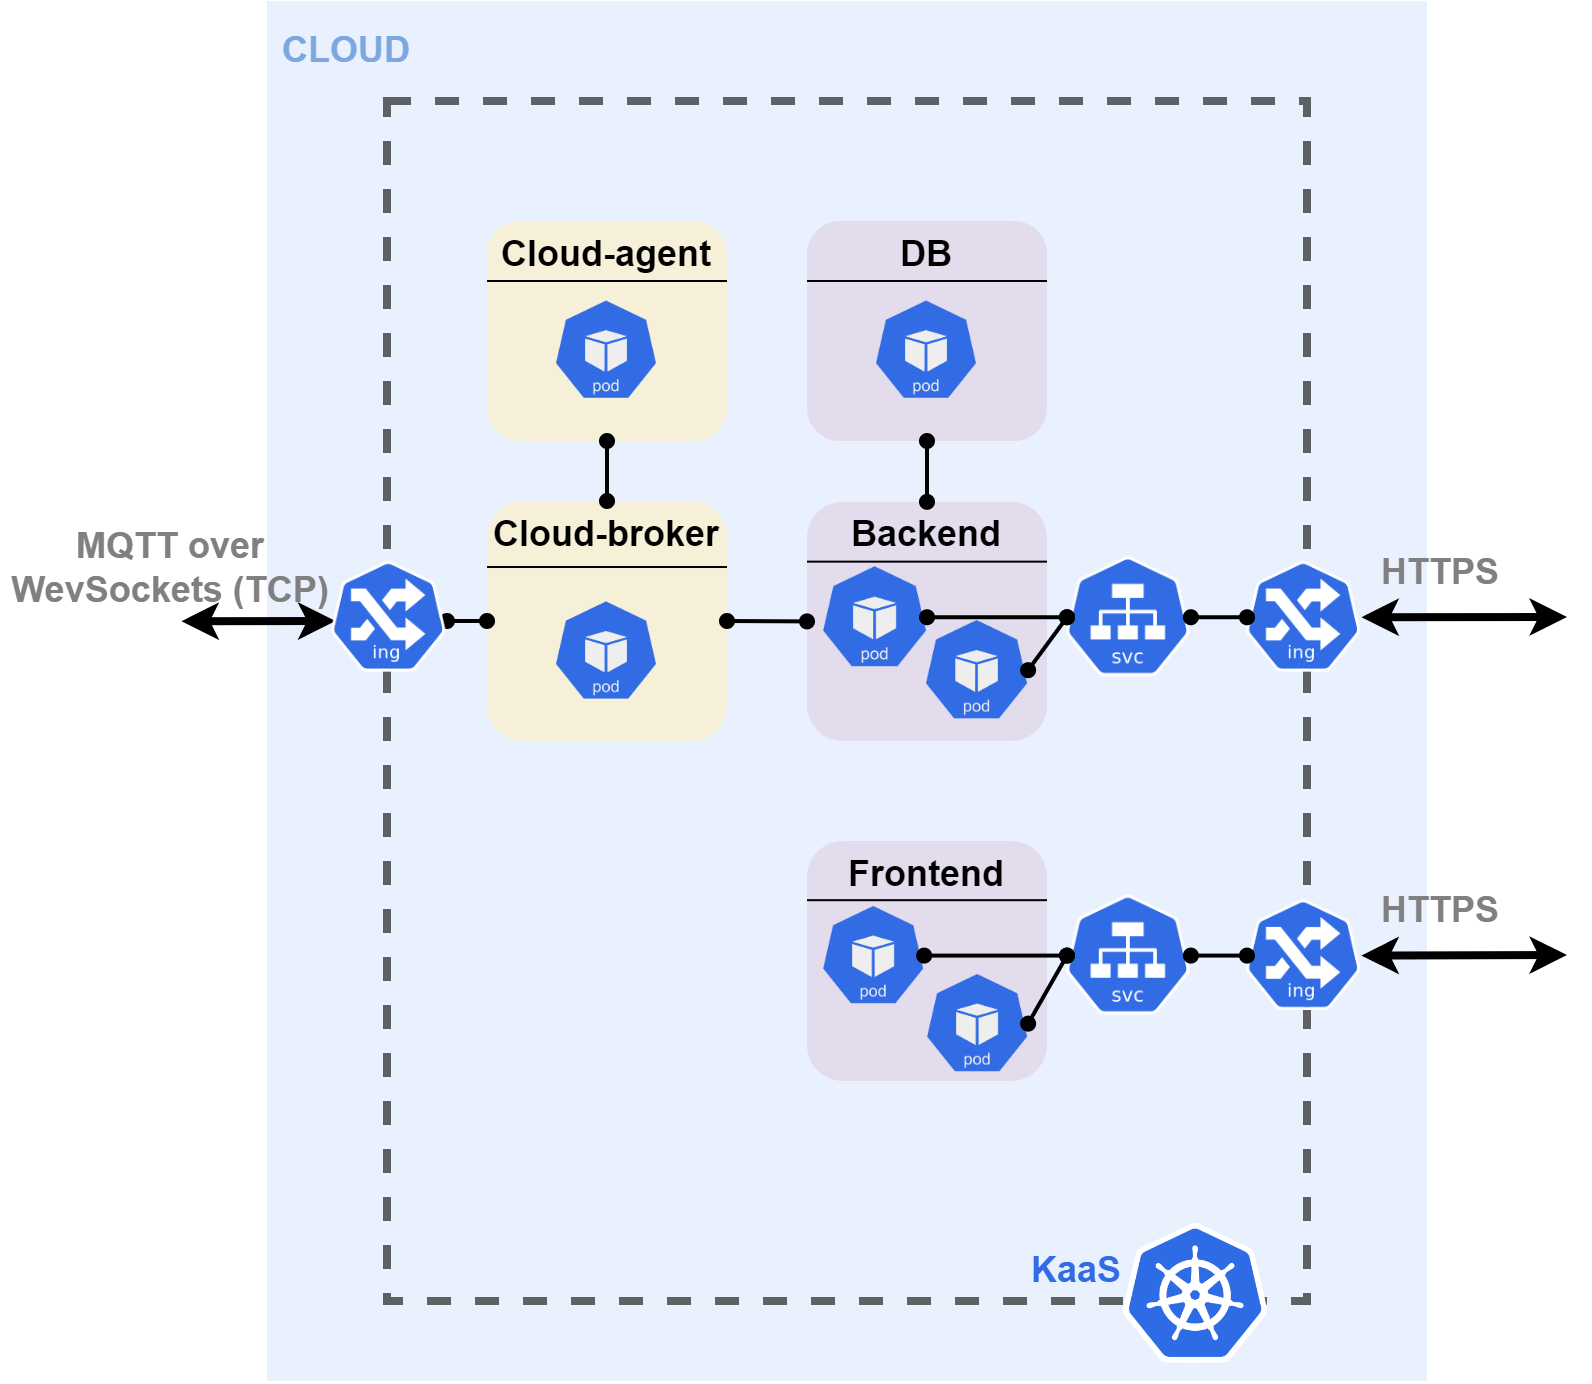
\includegraphics[width=0.8\textwidth]{pictures/cloud_services.png}
    \caption{ Cloud services system design }
    \label{fig:cloud_services}
\end{figure}

Three endpoints are exposed to external traffic(from outside of the cluster): two HTTP/HTTPS endpoints for the Backend and Frontend and one WebSocket endpoint for the MQTT messages send to the cloud broker.
HTTP/HTTPS traffic is being served via ingress resources in the cluster it is forwarded via reverse proxy to Kubernetes service which distributes the request among the pods. The default ingress resource is designed to only serve HTTP/HTTPS request and do not allow any other protocol. For MQTT protocol which is transported over TCP NodePort would have to be used to expose service to the outside world which maps pod ports to ports of the node in a cluster. Some cloud providers disallow usage of NodePorts, therefore more flexible option was chosen which is bootstrapping MQTT protocol over WebSockets and using ingress resources to handle external traffic coming to the cluster.
